% !TeX root = ../thuthesis-example.tex

% Your chapter title here
% Please make sure that the title is in CAPITALS
% All section and subsection headings, use capital letters where required
\chapter{INTRODUCTION}

\section{Problem definition}

Internet of Things (IoT) is expected to connect hundreds of billions of devices in less than a decade (\cite{simiscuka_synchronisation_2018}), with tens of billions of connected IoT devices already exist in the world. This number is anticipated to keep increasing as Internet connectivity has become a standard feature for a significant number of electronic devices (\cite{hu_virtual_2021}). Many companies, such as Huawei, Baidu, Alibaba, Tencent, Google, Intel, etc., already provide their solutions for operating with data coming from IoT devices. Although most of these products are restricted to be used only with the limited types or models of IoT devices, companies may come to the standardization of IoT devices in the next few years. Nowadays, most consumer IoT devices can be controlled by popular Smart assistants, such as Apple Siri, Amazon Alexa, Tencent Xiaowei, etc., or by SDKs, such as Apple HomeKit. Unified solutions make it possible to control all the devices using a phone, computer, or Smart Speaker.

On the other hand, controlling the IoT devices by smartphones and Smart speakers does not provide the best user experience. The interaction techniques are limited: even though the processing power per energy consumption has increased dramatically, and it is possible to have the processing power of high-performance PC of the 1990s in tiny devices, such as smartwatches, there is no freedom of movement and data sharing. Even though 5G networks partly solve the issue, for example, by making it possible to create Internet of Vehicle (IoV), the transmission bandwidth is still limited, causing severe safety consequences (\cite{hu_virtual_2021}). For example, when computations for interaction techniques, such as hand gesture recognition, can not be performed on the IoT device due to its limited computing power, the sensing data can be transferred to the server, analyzed, and only after sent back to the sensing device to provide output for the user.

The sixth-generation (6G) mobile network is expected to cast high-speed and high-efficiency transmission standards to adapt to the further development of new applications (\cite{liao_information-centric_2021}; \cite{huang_survey_2019}). It is expected for 6G network to be an evolution of 5G network and, therefore, provide faster data sharing between the devices, which will help overcome the issues stated in the previous paragraph. As soon as it becomes possible, the companies, which adapt their solutions for the new standards faster, will be more advanced in the IoT market. Development speed, in this case, is one of the most important factors for companies' success.

Nowadays, the standard way of integrating IoT devices in the development stage inside the existing environment is to either use their virtual (or digital) twins or build prototypes. In the first case, interaction with such devices is performed through a 2D interface, with a very rough simulation of the user behavior, which leads to further underestimations. In the second case, creating a prototype requires waiting for the IoT device's modeling, sending the schemes to the manufacturers, and then waiting for the prototype to be delivered. In both cases, the disadvantages lead to the possibility of losing the market, either because of lack of usability or because of being too late to enter the market, already taken by the competitors. Companies and researchers need an instrument to devoid these disadvantages and integrate the prototypes of devices inside the existing real-world IoT environment.

In this study, a solution for this issue is proposed: a platform for developing new IoT devices. The following section describes how using another perspective technology can help create the platform defined above.

\section{Research idea and tasks}

The problem of defining an instrument for having research on the new types of IoT devices and integrating such devices inside the existing real-world environments, which was introduced in the previous section, requires a solution, which can provide, at first, integration of real-world devices, and, at second, interaction with virtual devices.

Like IoT, Virtual reality (VR), together with AR, is considered one of the essential high-throughput application-level requirements of 6G. The biggest companies, such as Facebook, invest billions in AR and VR research. Nearly 10000 employees, almost 20% of the company staff, work on research in this field (link: https://www.theverge.com/2021/3/12/22326875/facebook-reality-labs-ar-vr-headcount-report TODO: put in the references). Research papers on applying Virtual reality into almost every area can be found, such as games, education, healthcare, or industry.

Companies selling Virtual Reality Headsets provide powerful APIs for integrating their devices inside different 3D engines \footnote{The Virtual reality market and 3D engine to be used in the research are further discussed in the next chapter.}. Researchers can use these interfaces to create a platform for interacting with virtual IoT devices.

The research idea is to integrate Virtual reality headsets into the IoT environment. In the 6G era, it will be possible to send large amounts of data with much smaller latency and much higher speed than the speed of 5G networks. Wi-Fi 6 (802.11ax standard) already provides acceptable results for high-quality streaming from VR headsets to the server for local scenarios.

Nevertheless, only using Virtual reality headsets does not solve the issue defined in the previous section. The research task is to define a layer between a real-world IoT environment and the user as a researcher to construct new IoT devices. 

\begin{figure}
  \centering
  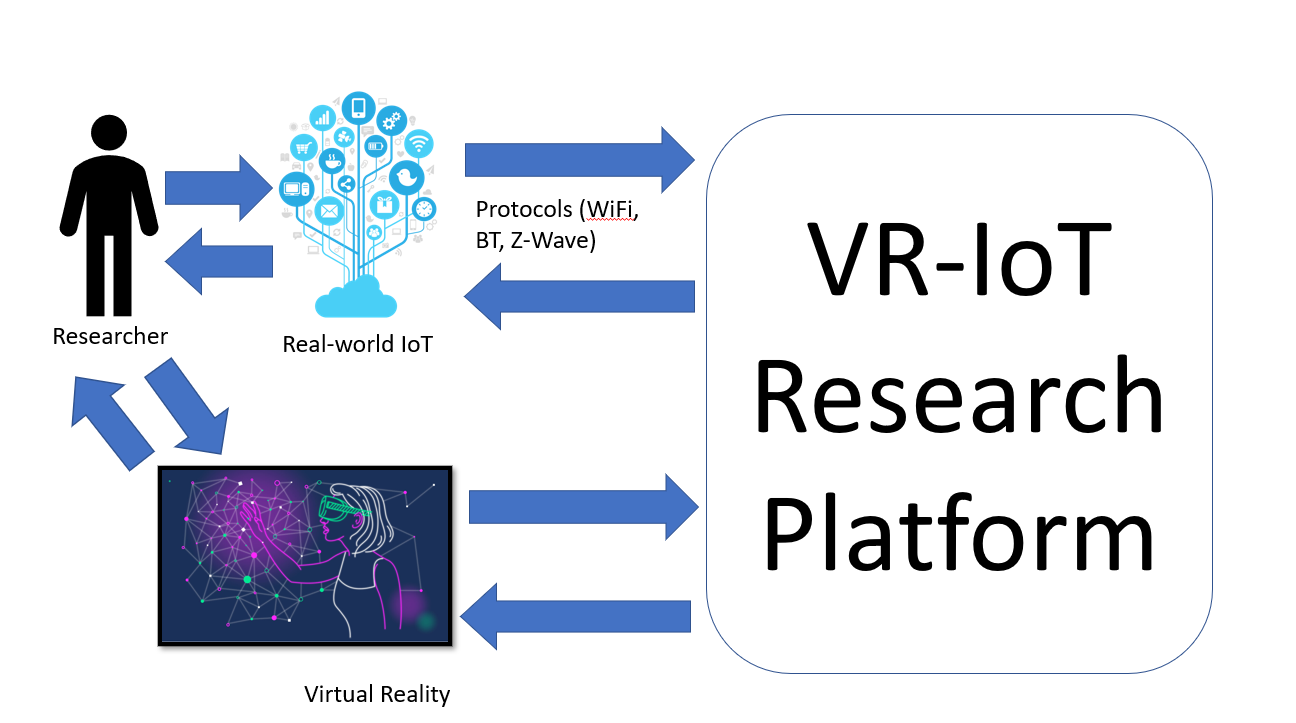
\includegraphics[width=0.9\linewidth]{figures/VR-IoTResearchPlatformLayer.png}
  \caption{VR-IoT Research Platform layer}
  \label{fig:VR-IoTResearchPlatformLayer-figure}
\end{figure}

In Chapter 3, the author proposes a prototype for the platform, with its evaluation in Chapter 4. In Chapters 5 and 6, important assumptions were made on how the platform should be designed in terms of architecture and API to connect to the real-virtual world IoT devices.

Summarizing the problem definition and research idea:

\begin{itemize}
    \item Problem definition: There is no instrument for fast creating, testing, and integrating new IoT devices inside an existing real-world environment.  
    \item Research idea: Define a layer between real-world IoT devices and Virtual Reality. Create a prototype, evaluate the performance and usability and summarize the outputs to explain why the selected architecture can be used as the basis for the future product used to design new IoT devices.
\end{itemize}